\documentclass[12pt,a4paper]{report}
% Layout shared by the coursework reports in this repository.
\usepackage{fontspec}
\IfFontExistsTF{DejaVu Sans Mono}{\setmonofont[Scale=0.84]{DejaVu Sans Mono}}{}
\usepackage[vietnamese]{babel}
\usepackage[a4paper,margin=1in]{geometry}
\usepackage{amsmath,amssymb,mathtools,bm}
\usepackage{booktabs,tabularx,array,longtable}
\usepackage{graphicx,float}
\usepackage{enumitem}
\usepackage{fancyhdr,setspace,titlesec,caption,microtype,needspace,etoolbox}
\usepackage[hidelinks]{hyperref}

\setstretch{1.15}
\setlength{\parskip}{0.45em}
\setlength{\parindent}{0pt}
\setlength{\headheight}{16pt}
\setcounter{tocdepth}{2}
\setcounter{secnumdepth}{3}
\emergencystretch=2em

\captionsetup{font=small,labelfont=bf}
\numberwithin{equation}{chapter}

\titleformat{\chapter}[display]
  {\normalfont\bfseries}
  {\filleft\Large\chaptertitlename\ \thechapter}
  {0.35em}
  {\filright\huge}
  [\vspace{0.4em}\titlerule]
\titlespacing*{\chapter}{0pt}{-10pt}{22pt}
\titleformat{\section}{\Large\bfseries}{\thesection}{0.6em}{}
\titleformat{\subsection}{\large\bfseries}{\thesubsection}{0.6em}{}
\titleformat{\subsubsection}{\normalsize\bfseries}{\thesubsubsection}{0.6em}{}

\preto\section{\Needspace{5\baselineskip}}{}
\preto\subsection{\Needspace{4\baselineskip}}{}
\preto\subsubsection{\Needspace{3\baselineskip}}{}

\newcommand{\CourseReportHeader}[1]{%
  \pagestyle{fancy}%
  \fancyhf{}%
  \fancyhead[L]{\small\nouppercase{\leftmark}}%
  \fancyhead[R]{\small #1}%
  \fancyfoot[C]{\thepage}%
  \fancypagestyle{plain}{%
    \fancyhf{}%
    \fancyhead[L]{\small\nouppercase{\leftmark}}%
    \fancyhead[R]{\small #1}%
    \fancyfoot[C]{\thepage}%
  }%
}

\newcommand{\R}{\mathbb{R}}
\newcommand{\norm}[1]{\left\lVert #1 \right\rVert}
\newcommand{\code}[1]{\texttt{\detokenize{#1}}}

% Arguments: logo, report type, course, title, author label, metadata rows, date.
\newcommand{\CourseCover}[7]{%
  \hypersetup{pageanchor=false}%
  \begin{titlepage}
    \centering
    \vspace*{0.5cm}
    {\normalsize\bfseries ĐẠI HỌC QUỐC GIA THÀNH PHỐ HỒ CHÍ MINH\par}
    {\normalsize\bfseries TRƯỜNG ĐẠI HỌC BÁCH KHOA\par}
    {\normalsize\bfseries KHOA KHOA HỌC VÀ KỸ THUẬT MÁY TÍNH\par}
    \vspace{0.6cm}
    \includegraphics[width=0.2\textwidth]{#1}\par
    \vspace{0.7cm}
    {\large\bfseries #2\par}
    \vspace{0.35cm}
    {\normalsize\textbf{#3}\par}
    {\small Học kỳ 261 · Năm học 2026–2027\par}
    \vspace{0.45cm}
    {\LARGE\bfseries #4\par}
    \vspace{0.6cm}
    {\normalsize\bfseries #5\par}
    \vspace{0.35cm}
    {\small\begin{tabular}{@{}ll@{}}#6\end{tabular}\par}
    \vfill
    {\small\bfseries Thành phố Hồ Chí Minh, #7\par}
  \end{titlepage}
  \pagenumbering{roman}%
  \hypersetup{pageanchor=true}%
}

\newcommand{\CourseFrontChapter}[1]{%
  \chapter*{#1}%
  \addcontentsline{toc}{chapter}{#1}%
  \markboth{#1}{#1}%
}

\newcommand{\CourseAbstract}[1]{%
  \CourseFrontChapter{Tóm tắt}%
  #1\par
}

\newcommand{\CourseOverview}[1]{%
  \CourseFrontChapter{Tổng quan báo cáo}%
  \begingroup
  \renewcommand{\arraystretch}{1.3}%
  \begin{tabularx}{\textwidth}{@{}>{\bfseries\raggedright\arraybackslash}p{3.3cm}>{\raggedright\arraybackslash}X@{}}
    #1
  \end{tabularx}
  \endgroup
}

% Omit the figure list for a report containing only tables.
\newcommand{\CourseContents}[1][\listoffigures]{%
  \tableofcontents
  #1%
  \listoftables
  \clearpage
  \pagenumbering{arabic}%
}

\CourseReportHeader{CO5085 · A2}
\hypersetup{pdftitle={Phan doan anh voi phep tron dac trung theo bien},pdfauthor={Huynh Thanh Dat}}

\begin{document}
\CourseCover{assets/hcmut-logo.png}
  {BÁO CÁO BÀI TẬP LỚN A2}
  {CO5085 · Học sâu và ứng dụng trong thị giác máy tính}
  {Phân đoạn ảnh với phép trộn đặc trưng theo biên}
  {Sinh viên}
  {Huỳnh Thành Đạt & 2570161\\[0.5em]
   Giảng viên & Lê Thành Sách\\
              & Nguyễn Quốc Minh}
  {tháng 11 năm 2026}

\CourseAbstract{
PIDNet dùng thông tin biên để điều chỉnh tỷ lệ trộn đặc trưng chi tiết và ngữ cảnh trong phân đoạn ảnh. Thí nghiệm khảo sát cơ chế này trên Oxford-IIIT Pet bằng hai biến thể ResNet18 có cùng đầu dự đoán biên, lần lượt dùng hệ số trộn cố định và hệ số trộn theo vị trí. Sáu lượt huấn luyện, mỗi lượt 12 epoch trên đầy đủ tập train, cho mIoU trung bình $78{,}00\pm0{,}11$\% với trộn cố định và $77{,}82\pm0{,}03$\% với trộn theo biên. Chênh lệch ghép theo seed là $-0{,}18\pm0{,}12$ điểm phần trăm. IoU dải chuyển tiếp lần lượt đạt $55{,}15\pm0{,}39$\% và $55{,}02\pm0{,}13$\%. Đầu biên phân biệt được các vùng, nhưng dùng tín hiệu này để điều tiết phép trộn chưa cải thiện chất lượng phân đoạn trung bình.

}

\CourseOverview{
Bài toán & Phân đoạn vật thể, nền và dải chuyển tiếp trên Oxford-IIIT Pet.\\
Bài báo & PIDNet của Xu, Xiong và Bhattacharyya, IEEE/CVF CVPR 2023 \cite{pidnet}.\\
Đối chứng & ResNet18 dùng chung kiến trúc và giám sát biên. Hai biến thể lần lượt dùng tỷ lệ 50/50 và hệ số trộn theo vị trí.\\
Phép đo & mIoU, macro-Dice và IoU theo vùng trên 3.669 ảnh test. Mỗi biến thể chạy ba seed.\\
Kết quả chính & mIoU của trộn cố định và trộn theo biên lần lượt là 78,00\% và 77,82\%.\\
Đối chiếu & Mức thay đổi mIoU trong các phép ablation công bố và thí nghiệm A2.\\
}

\CourseContents

\chapter{Câu hỏi nghiên cứu}
Phân đoạn ảnh yêu cầu xác định vùng của từng điểm ảnh. Đặc trưng ở độ phân giải thấp giúp nhận ra vật thể trong ngữ cảnh chung, nhưng khi đưa trở lại lưới ảnh, chúng có thể làm mờ đường viền. Đặc trưng ở độ phân giải cao giữ nhiều chi tiết hơn và cũng dễ phản ứng với hoa văn của lông hoặc nền. Hai nguồn thông tin vì vậy có giá trị khác nhau ở phần trong của vật thể và vùng chuyển tiếp giữa vật thể với nền.

Thí nghiệm khảo sát ý tưởng trộn đặc trưng theo bản đồ biên trong PIDNet của Xu, Xiong và Bhattacharyya \cite{pidnet}. Câu hỏi thực nghiệm là liệu phép trộn thay đổi theo vị trí có tăng IoU của dải chuyển tiếp trên Oxford-IIIT Pet khi cả hai mô hình đã được giám sát bằng nhãn vùng này. IoU theo từng vùng được phân tích cùng mIoU và Dice để xác định thay đổi ở dải chuyển tiếp có đi kèm thay đổi ở vật thể và nền hay không.

\chapter{Phân tích PIDNet}
\section{Giới hạn của các mạng hai nhánh}

Trong phân đoạn thời gian thực, giảm kích thước bản đồ đặc trưng giúp giảm chi phí, nhưng việc giảm mẫu sớm làm mất thông tin định vị. Một pixel trong bản đồ sâu có thể tổng hợp cả hai phía của đường viền. Khi nội suy trở lại lưới ảnh, tín hiệu đó có thể lan sang vùng bên cạnh, làm mờ biên hoặc xóa một vật thể nhỏ giữa vùng nền lớn. Các bộ mã hóa dùng tích chập giãn có thể giữ lưới dày hơn ở những tầng sâu, với chi phí bộ nhớ và độ trễ phụ thuộc phần cứng.

BiSeNet \cite{bisenet} xử lý sự đánh đổi này bằng một luồng giữ chi tiết không gian và một luồng tổng hợp ngữ cảnh. DDRNet \cite{ddrnet} duy trì hai độ phân giải và trao đổi thông tin giữa chúng qua nhiều tầng. Theo phân tích của PIDNet, ngay cả khi nhánh chi tiết còn giữ được một đoạn biên, việc cộng hai bản đồ có thể làm đáp ứng ngữ cảnh mạnh lấn át tín hiệu cục bộ. Chẳng hạn ở mép một vật thể mảnh, phần lớn trường tiếp nhận của nhánh sâu có thể nằm trong nền. Nhãn nền có thể lan qua mép khi đặc trưng hai nhánh được trộn cùng một cách ở mọi vị trí.

\section{Phép tương tự với điều khiển PID}

Trong bộ điều khiển, thành phần tỉ lệ P phản ứng với sai số hiện tại, I tích lũy sai số và D phản ứng với sự thay đổi của sai số. Ở miền tần số rời rạc, bỏ qua hệ số khuếch đại và xét $0<\omega\leq\pi$, độ lớn đáp ứng của tích phân và vi phân lần lượt là
\[
 \lvert H_I(e^{j\omega})\rvert
 = \frac{1}{2\lvert\sin(\omega/2)\rvert},
 \qquad
 \lvert H_D(e^{j\omega})\rvert
 = 2\lvert\sin(\omega/2)\rvert.
\]
Tích phân nhấn mạnh biến thiên chậm, còn vi phân đáp ứng mạnh khi tín hiệu đổi nhanh. Trên mô hình một chiều của paper, nhánh chi tiết có trường tiếp nhận tập trung gần vị trí đang xét, trong khi nhánh ngữ cảnh tổng hợp trên vùng rộng hơn. Tác giả liên hệ hai nhánh với P và I, rồi dùng hiện tượng đáp ứng vượt mức của PI để giải thích trực giác về sự lan nhãn qua biên. Thành phần D gợi ý một tín hiệu bổ sung có thể làm thay đổi phép trộn tại nơi nhãn chuyển nhanh.

\begin{table}[htbp]
\centering
\begin{tabularx}{\linewidth}{@{}lXX@{}}
\toprule
Nhánh & Thông tin chính & Vai trò khi tổng hợp\\
\midrule
P & Chi tiết không gian trên lưới tương đối dày. & Giữ hình dạng và vị trí của đường viền.\\
I & Ngữ cảnh từ tầng sâu và khối gộp hình tháp. & Ổn định nhãn trong vùng đồng nhất.\\
D & Tín hiệu chuyển lớp được giám sát bằng nhãn biên. & Điều chỉnh trọng số dành cho P và I theo vị trí.\\
\bottomrule
\end{tabularx}
\caption{Vai trò của ba nhánh trong PIDNet.}
\label{tab:branches}
\end{table}

PIDNet dùng một nhánh học từ dữ liệu để định vị biên ngữ nghĩa như mô tả trong Bảng~\ref{tab:branches}. Các đáp ứng tần số trên mô tả bộ điều khiển tuyến tính, còn các nhánh tích chập thực tế có chuẩn hóa, hàm kích hoạt và các kết nối chéo. Trong Bag, D cung cấp hệ số trộn cho hai luồng đặc trưng.

\section{Trao đổi thông tin và hàm mục tiêu}

Nhánh I gửi thông tin ngữ nghĩa sang P qua Pag và bổ sung đặc trưng cho D bằng phép cộng. Pag chiếu hai vector tại cùng vị trí, lấy tích vô hướng và áp dụng sigmoid để điều chỉnh mức tiếp nhận ngữ cảnh của P. PAPPM tổng hợp ngữ cảnh qua các nhánh gộp song song trong PIDNet-S/M. Ở cuối mạng, Bag sử dụng tín hiệu của D để điều tiết hai luồng. Với đặc trưng chi tiết $P$, ngữ cảnh $I$ và biểu diễn biên $D$, biểu thức của Bag có dạng
\[
    a=\sigma(D),\qquad
    Y=f_{\mathrm{out}}\big(a\odot P+(1-a)\odot I\big).
\]
Hệ số $a$ lớn tăng đóng góp của P ở vùng chuyển lớp. Ở vùng tương đối đồng nhất, I cung cấp ngữ cảnh để ổn định nhãn. Light-Bag dùng một phép kết hợp với các tích chập $1\times1$ để giảm độ trễ trong biến thể nhẹ.

Hàm mục tiêu của paper gồm cross-entropy ở đầu ra phụ và đầu ra chính, BCE có trọng số để giám sát nhánh D, cùng một cross-entropy có nhận biết biên. Thành phần cuối chỉ tính tại các vị trí có đáp ứng biên vượt ngưỡng $0{,}8$ theo thiết lập của tác giả. Nhánh D vừa nhận tín hiệu trực tiếp từ nhãn biên, vừa tham gia quyết định đặc trưng được đưa vào bộ phân loại điểm ảnh.

\section{Thí nghiệm gốc và phạm vi kết luận}

Bài báo đánh giá mIoU trên Cityscapes, CamVid và PASCAL Context. Với Cityscapes, tác giả dùng ảnh $2048\times1024$ và báo cáo PIDNet-S đạt 78,6\% mIoU trên tập test, ở 93,2 FPS trong phép đo với RTX 3090, batch 1 và gộp BatchNorm vào tích chập. Trên CamVid, mô hình này đạt 80,1\% mIoU sau khi khởi tạo từ trọng số Cityscapes. Kết quả này gắn với điều kiện khởi tạo từ Cityscapes. PIDNet-L đạt 80,6\% trên Cityscapes test ở 31,1 FPS, phản ánh chi phí của biến thể lớn. Trên PASCAL Context, PIDNet-L đạt 51,9\% mIoU ở giao thức 59 lớp với suy luận đa tỷ lệ và lật ảnh, so với 54,0\% của HRNet-W48 trong Bảng~7. Kết quả này cho thấy lợi thế phụ thuộc bộ dữ liệu và chế độ suy luận.

Đối chứng trong Bảng~1 của paper cho thấy thêm nhánh biên và Bag vào BiSeNet dùng ResNet18 tăng mIoU trên tập validation của Cityscapes từ 75,4\% lên 76,7\%, đồng thời giảm tốc độ từ 63,2 xuống 52,1 FPS. Hai thành phần được thêm cùng lúc nên mức tăng này chưa tách riêng tác dụng của phép trộn. Bảng~3 giữ PAPPM và so sánh phép cộng với Light-Bag trên PIDNet-S. mIoU tăng từ 78,4\% lên 78,8\%, còn FPS giảm từ 97,8 xuống 93,2. Kết quả thể hiện sự đánh đổi giữa độ chính xác và tốc độ ngay trong cùng một họ kiến trúc.

Trong chuỗi ablation ở Bảng~4, việc bổ sung loss biên có trọng số tăng mIoU từ 78,8\% lên 79,9\% khi loss ngữ nghĩa phụ đã có. Tác giả cũng lưu ý mô hình cần nhãn biên đủ chính xác. Các bảng mIoU gộp toàn ảnh nên khó xác định phần cải thiện nằm sát biên, trên vật thể nhỏ hay ở vùng trong. Phép đo FPS còn phụ thuộc độ phân giải, phần cứng và cấu hình suy luận. Ở ảnh thú cưng, lông, bóng đổ và nền có hoa văn tạo nhiều biến thiên cục bộ; đáp ứng cao ở các vùng này có thể dẫn đến ưu tiên chi tiết ngay cả khi nhãn thực thuộc vùng nền. Thí nghiệm đo riêng IoU dải chuyển tiếp để khảo sát sai số tại vùng này.

\chapter{Dữ liệu và thiết lập thực nghiệm}
\section{Dữ liệu và phân tích khám phá}
Oxford-IIIT Pet có 7.349 ảnh với 37 giống chó và mèo, kích thước và tư thế đa dạng \cite{pets,petsdata}. Mỗi ảnh có trimap, trong đó giá trị 1 là vật thể, 2 là nền và 3 là vùng chưa phân loại. Báo cáo gọi nhãn 3 là \emph{dải chuyển tiếp} và dùng nó làm tín hiệu gần đúng cho biên. Nhãn giống chỉ phục vụ việc chia tập. Tập dữ liệu được công bố theo CC BY-SA 4.0 trên trang của Oxford. Quyền tác giả ảnh thuộc về chủ sở hữu gốc.

Từ 3.680 ảnh trong tập huấn luyện/validation chính thức, chọn 10 ảnh mỗi giống làm tập validation bằng seed 2026. Phần còn lại gồm 3.310 ảnh dùng để cập nhật trọng số. Tập test chính thức gồm 3.669 ảnh được giữ riêng. Đối chiếu kích thước và pixel RGB giải mã không tìm thấy ảnh trùng chính xác giữa các tập; phép đối chiếu này chỉ phát hiện ảnh trùng pixel.

Trung vị chiều rộng và chiều cao ảnh gốc lần lượt là 500 và 375 pixel. Trên lưới dùng để huấn luyện, vật thể chiếm 30{,}23\% điểm ảnh có nhãn, nền chiếm 58{,}36\% và dải chuyển tiếp chiếm 11{,}41\%. Tỷ lệ dải chuyển tiếp theo từng ảnh có trung vị 10{,}91\% và khoảng tứ phân vị 8{,}64--13{,}77\%. BCE cân bằng duy trì đóng góp của dải chuyển tiếp vào loss phụ dù vùng này chiếm ít pixel hơn.


\begin{figure}[htbp]
\centering
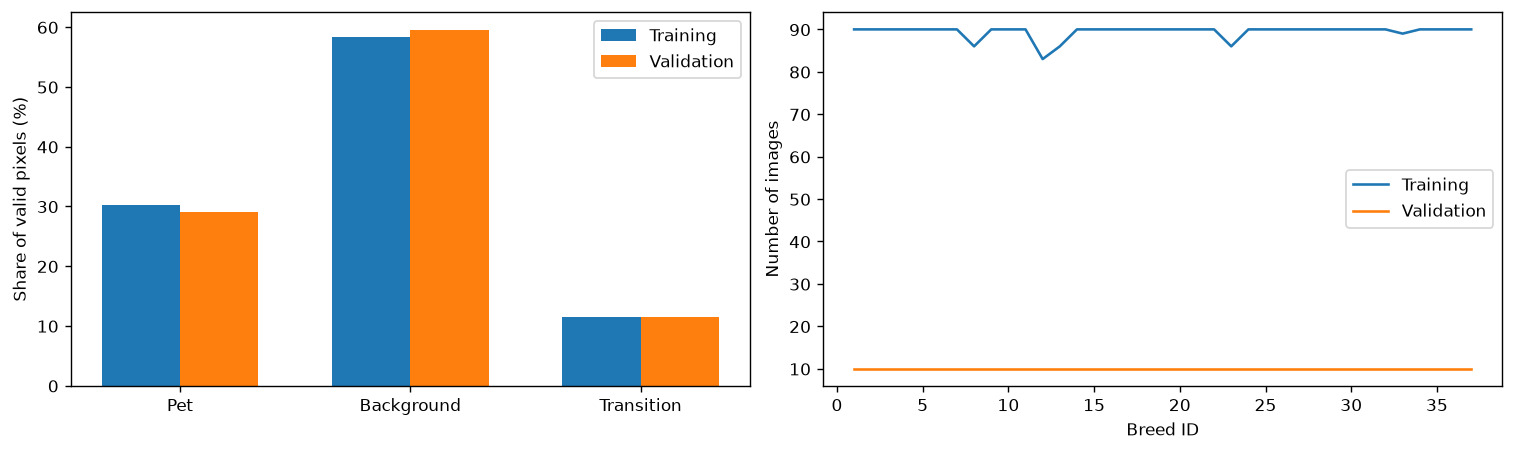
\includegraphics[width=\linewidth]{notebook-evidence/figures/notebook-1.png}
\caption{Tỷ lệ điểm ảnh theo nhãn và số ảnh theo giống ở tập train và validation. Tỷ lệ pixel được tính sau khi đưa ảnh về lưới thực nghiệm và bỏ vùng đệm.}
\label{fig:eda}
\end{figure}

\begin{figure}[htbp]
\centering
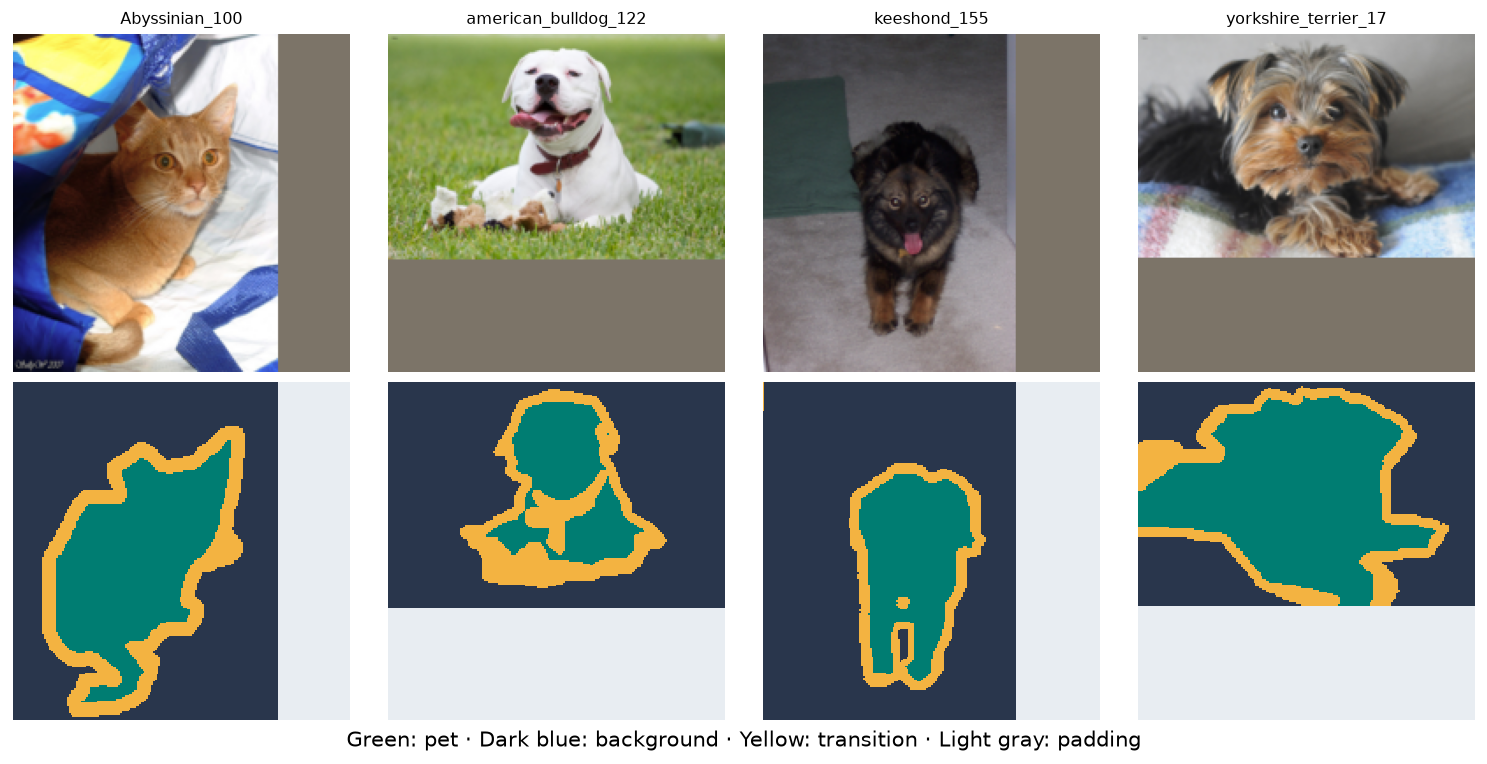
\includegraphics[width=\linewidth]{notebook-evidence/figures/notebook-2.png}
\caption{Bốn ảnh validation và trimap tương ứng. Xanh lục là vật thể, xanh đậm là nền, vàng là dải chuyển tiếp và xám nhạt là vùng đệm. Ảnh và trimap từ Oxford-IIIT Pet, CC BY-SA 4.0 \cite{petsdata}.}
\label{fig:trimaps}
\end{figure}

\section{Cài đặt và giao thức đánh giá}
\subsection{Tiền xử lý}

Cạnh dài của ảnh được nội suy về 192 pixel, giữ tỷ lệ khung hình và đệm bên phải hoặc phía dưới để có đầu vào $192\times192$. Ảnh RGB dùng nội suy song tuyến tính, còn trimap dùng láng giềng gần nhất để giữ giá trị nhãn. Nhãn đệm được bỏ qua trong hàm mục tiêu và phép đo. Tập huấn luyện xáo thứ tự và lật ngang đồng thời ảnh và mặt nạ với xác suất 0,5. Các tập validation và test dùng phép biến đổi cố định. Chuẩn hóa RGB sử dụng trung bình và độ lệch chuẩn ImageNet.

\subsection{Hai biến thể có cùng cấu trúc}

Hai mô hình dùng ResNet18 với trọng số ImageNet từ torchvision \cite{resnet,torchvision}. Đầu phân loại của ResNet18 được bỏ. Đặc trưng nông lấy từ \code{layer1} ở stride 4 và đặc trưng sâu lấy từ \code{layer4} ở stride 32. Hai nhánh được chiếu về 64 kênh; đặc trưng sâu được nội suy về lưới đặc trưng nông. Một đầu dự đoán biên trên đặc trưng nông xuất một logit $e$ tại mỗi vị trí.

\begin{table}[htbp]
\centering
\begin{tabularx}{\linewidth}{@{}lXX@{}}
\toprule
Biến thể & Phép trộn tại từng vị trí & Vai trò của đầu dự đoán biên\\
\midrule
Trộn cố định & $0{,}5P+0{,}5I$ & Học bằng hàm mất mát phụ.\\
Trộn theo biên & $\sigma(e)P+(1-\sigma(e))I$ & Học bằng hàm mất mát phụ và tham gia trộn đặc trưng.\\
\bottomrule
\end{tabularx}
\caption{Hai biến thể cùng số tham số, trọng số khởi tạo và giao thức huấn luyện.}
\label{tab:variants}
\end{table}

Bộ phân loại điểm ảnh giống nhau ở hai biến thể. Logit của ba vùng được nội suy về lưới ảnh trước khi tính loss và lấy nhãn có logit lớn nhất. Thí nghiệm giữ phép trộn theo sigmoid của Bag, dùng một hệ số chung cho mọi kênh và một bộ mã hóa ResNet18. Các khối Pag, PAPPM và nhánh D độc lập của PIDNet nằm ngoài cấu hình này. Đầu phụ và giám sát biên giống nhau ở hai biến thể, giúp cô lập việc đưa bản đồ biên vào phép trộn.

\subsection{Huấn luyện}

Với $\Omega$ là các điểm ảnh có nhãn, hàm mục tiêu là cross-entropy ba vùng cộng BCE cân bằng theo nhóm. Gọi $\Omega_b$ là dải chuyển tiếp, $\Omega_n$ là phần còn lại của $\Omega$, và $\ell_{\mathrm{BCE}}(e,y)$ là BCE tính trực tiếp từ logit. Khi hai nhóm đều có điểm ảnh,
\[
 L=L_{\mathrm{CE}}+0{,}25 L_b,\quad
 L_b=\frac{1}{2|\Omega_b|}\sum_{i\in\Omega_b}\ell_{\mathrm{BCE}}(e_i,1)
    +\frac{1}{2|\Omega_n|}\sum_{i\in\Omega_n}\ell_{\mathrm{BCE}}(e_i,0).
\]
Nếu một nhóm rỗng trong batch, đóng góp của nhóm đó bằng 0. Việc lấy trung bình riêng giúp dải chuyển tiếp vẫn đóng góp vào gradient dù chiếm ít điểm ảnh. Khác với loss có ngưỡng của PIDNet, thành phần CE ở đây luôn tính trên toàn bộ $\Omega$. Tín hiệu biên của bản trộn theo biên còn nhận gradient qua loss chính vì phép trộn khả vi.

Mỗi biến thể chạy 12 epoch với ba seed 42, 43 và 44. Batch size là 32. AdamW dùng hệ số suy giảm trọng số $10^{-4}$ và tốc độ học ban đầu $2\times10^{-4}$ cho bộ mã hóa, $10^{-3}$ cho các đầu mới. Tốc độ học giảm theo cosine sau mỗi epoch. Vòng lặp gọi trực tiếp forward, tính loss, lan truyền ngược và cập nhật trọng số. Sáu lượt huấn luyện được thực hiện trực tiếp từ notebook trên NVIDIA GeForce RTX 5090, BF16 autocast với loss tính bằng FP32, 4 worker tải dữ liệu và 4 luồng CPU của PyTorch. Môi trường gồm Python 3.12.12, PyTorch 2.10.0, torchvision 0.25.0 và CUDA 13.0.

\subsection{Chọn checkpoint và chỉ số đánh giá}

Mỗi lượt chọn checkpoint có mIoU trên tập validation cao nhất. Khi bằng nhau, chọn epoch sớm hơn. Tập test chỉ được đánh giá sau khi cả sáu lượt huấn luyện hoàn tất và giao thức đã cố định.

Với mỗi lớp $c$, lấy $TP_c$, $FP_c$ và $FN_c$ từ ma trận đếm điểm ảnh trên toàn tập. Các chỉ số được tính như sau:
\[
  \mathrm{IoU}_c=\frac{TP_c}{TP_c+FP_c+FN_c},\qquad
  \mathrm{Dice}_c=\frac{2TP_c}{2TP_c+FP_c+FN_c}.
\]
mIoU và macro-Dice là trung bình đều trên ba lớp. Cách gộp này cho dải chuyển tiếp cùng trọng số với các lớp lớn, dù số điểm ảnh mỗi lớp khác nhau. IoU riêng của dải chuyển tiếp dùng đúng nhãn trimap ở lưới $192\times192$ và phản ánh độ khớp vùng. Sai lệch biên tính bằng khoảng cách trên ảnh gốc nằm ngoài phép đo.

\chapter{Kết quả thực nghiệm}
\section{So sánh các biến thể}
\begin{table}[htbp]\centering\small
\begin{tabular}{@{}lrrrrr@{}}\toprule
Biến thể & mIoU & Dice & IoU vật thể & IoU nền & IoU chuyển tiếp\\\midrule
Trộn cố định & $78{,}00 \pm 0{,}11$ & $86{,}62 \pm 0{,}10$ & $86{,}17 \pm 0{,}10$ & $92{,}68 \pm 0{,}03$ & $55{,}15 \pm 0{,}39$\\
Trộn theo biên & $77{,}82 \pm 0{,}03$ & $86{,}51 \pm 0{,}02$ & $85{,}89 \pm 0{,}15$ & $92{,}55 \pm 0{,}05$ & $55{,}02 \pm 0{,}13$\\
\bottomrule\end{tabular}
\caption{Kết quả trên tập test theo phần trăm, trình bày trung bình và độ lệch chuẩn mẫu qua ba seed.}
\label{tab:results}\end{table}

\begin{table}[htbp]\centering\small
\begin{tabular}{@{}lrrrr@{}}\toprule
Biến thể & Validation mIoU (\%) & Epoch được chọn & Thời gian (s) & Đỉnh (MiB)\\\midrule
Trộn cố định & $77{,}46 \pm 0{,}10$ & 10, 8, 9 & $8{,}8 \pm 0{,}3$ & $559{,}7 \pm 1{,}2$\\
Trộn theo biên & $77{,}44 \pm 0{,}08$ & 10, 8, 9 & $8{,}6 \pm 0{,}0$ & $572{,}2 \pm 0{,}0$\\
\bottomrule\end{tabular}
\caption{Chi phí của 12 epoch và kết quả trên tập validation. Epoch theo thứ tự seed 42, 43, 44. Thời gian gồm tải batch và cập nhật trọng số. Mức cấp phát GPU cực đại bao gồm lượt đánh giá trên tập validation.}
\label{tab:cost}\end{table}


Cả hai biến thể chọn các epoch 10, 8 và 9 theo thứ tự seed 42, 43 và 44 trong lịch 12 epoch. Hình~\ref{fig:curves} cho thấy loss huấn luyện tiếp tục giảm đến cuối lịch, trong khi mIoU trên tập validation chững lại quanh 77\% sau epoch 8. Các đường validation gần nhau nên mức khác biệt được xem thêm qua từng cặp seed và từng vùng trên tập test.

\begin{figure}[htbp]
\centering
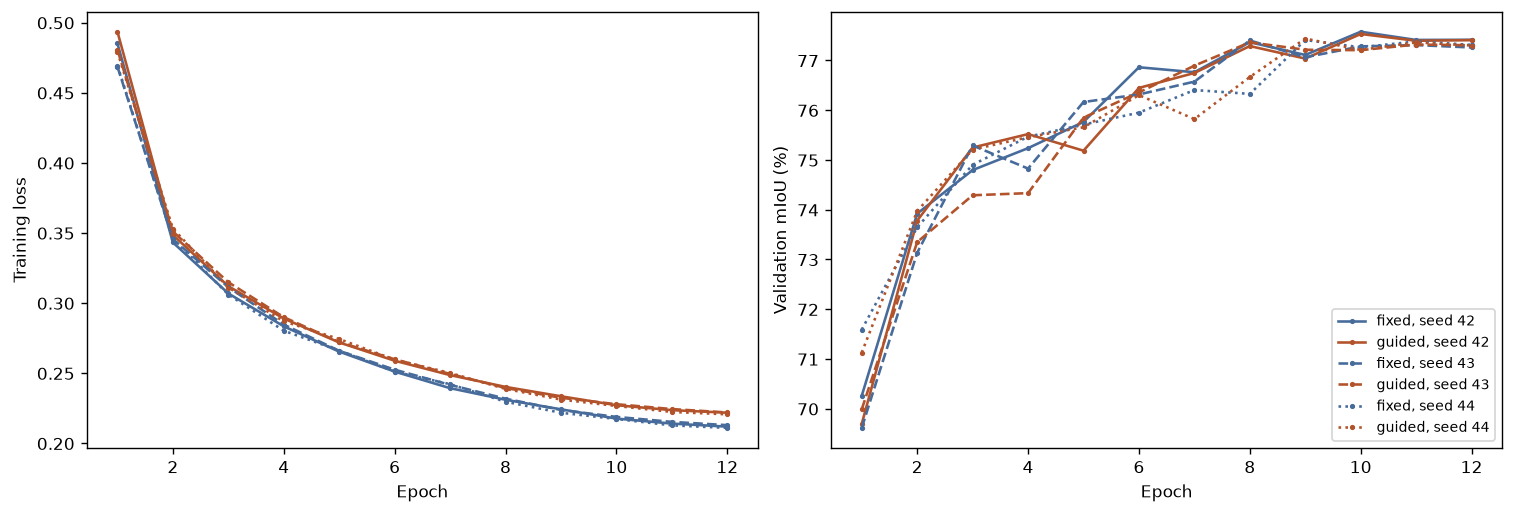
\includegraphics[width=\linewidth]{notebook-evidence/figures/notebook-3.png}
\caption{Loss huấn luyện và mIoU trên tập validation theo epoch của sáu lượt chạy. Màu thể hiện biến thể, kiểu nét phân biệt seed; mỗi đường là một lượt thực nghiệm.}
\label{fig:curves}
\end{figure}

\begin{figure}[htbp]
\centering
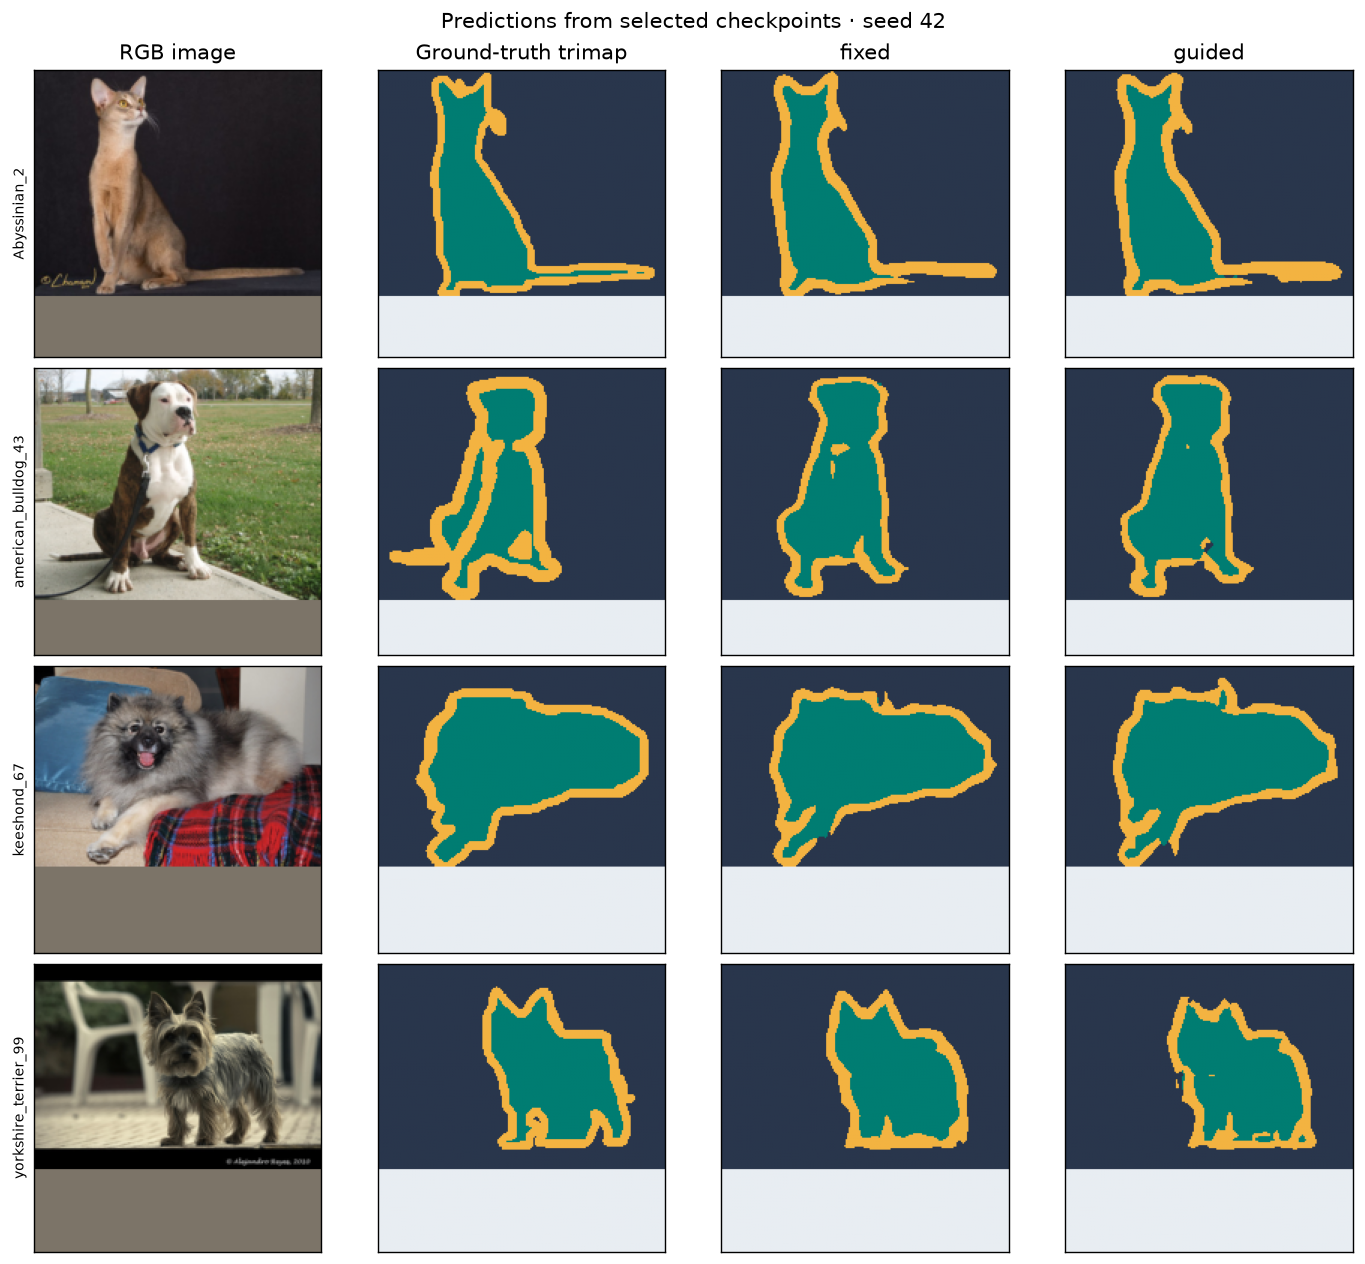
\includegraphics[width=0.95\linewidth,height=0.75\textheight,keepaspectratio]{notebook-evidence/figures/notebook-5.png}
\caption{Bốn ảnh test tại seed 42, lần lượt gồm ảnh RGB, trimap, dự đoán trộn cố định và dự đoán trộn theo biên. Xanh lục là vật thể, xanh đậm là nền, vàng là dải chuyển tiếp. Ảnh và trimap từ Oxford-IIIT Pet, CC BY-SA 4.0 \cite{petsdata}.}
\label{fig:examples}
\end{figure}

\begin{figure}[htbp]
\centering
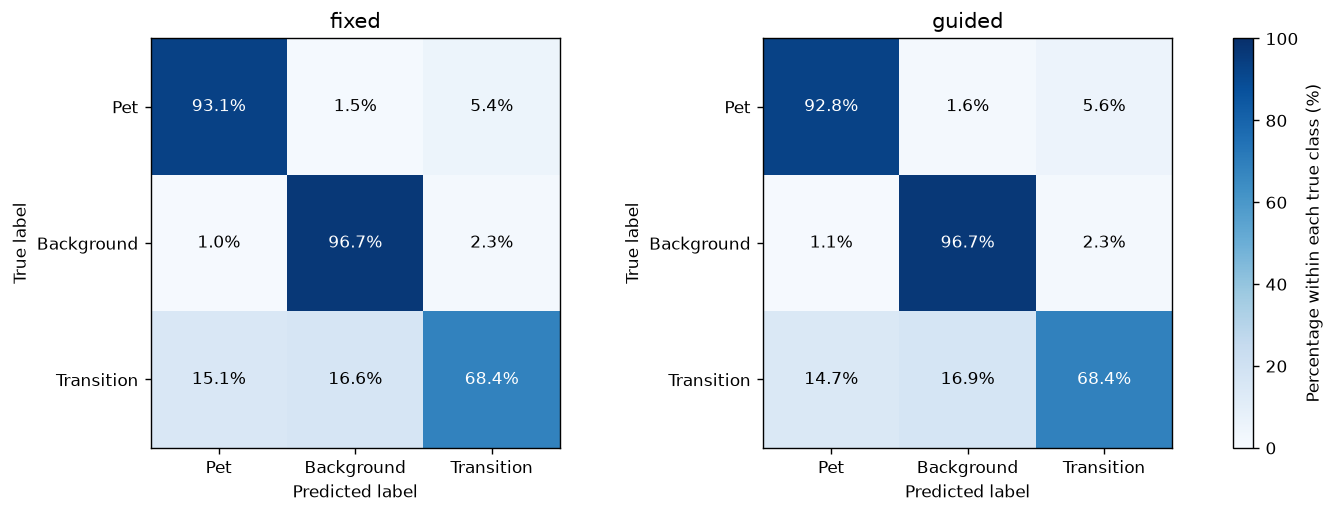
\includegraphics[width=\linewidth]{notebook-evidence/figures/notebook-4.png}
\caption{Ma trận nhầm lẫn theo pixel, gộp ba seed của mỗi biến thể. Hàng là nhãn thực, cột là nhãn dự đoán; tỷ lệ được chuẩn hóa theo từng hàng.}
\label{fig:confusion}
\end{figure}

\subsection{Độ chính xác theo vùng}

Hai mô hình cùng có 11.302.116 tham số được huấn luyện. So với trộn cố định, trộn theo biên thay đổi mIoU $-0{,}18\pm0{,}12$ điểm phần trăm và macro-Dice $-0{,}11\pm0{,}09$ điểm phần trăm khi ghép theo seed. mIoU giảm ở cả ba cặp, lần lượt $0{,}16$, $0{,}31$ và $0{,}07$ điểm phần trăm. Mức giảm IoU trung bình lớn nhất thuộc vùng vật thể ($0{,}28$ điểm phần trăm), tiếp đến là nền và dải chuyển tiếp (đều khoảng $0{,}13$ điểm phần trăm). IoU dải chuyển tiếp tăng $0{,}11$ điểm phần trăm ở seed 44, nhưng giảm ở hai seed còn lại. Ba cặp seed chỉ mô tả độ dao động trong thiết lập đã khảo sát.

Dải chuyển tiếp vẫn là vùng khó nhất, với IoU khoảng 55\%, thấp hơn IoU vật thể khoảng 86\% và IoU nền trên 92\%. Ma trận nhầm lẫn ở Hình~\ref{fig:confusion} cho thấy khoảng 68,4\% pixel thực của dải chuyển tiếp được nhận đúng ở cả hai biến thể. Với bản cố định, 15,1\% bị gán thành vật thể và 16,6\% thành nền; các tỷ lệ tương ứng của bản theo biên là 14,7\% và 16,9\%. Tỷ lệ nhận đúng dải chuyển tiếp gần bằng nhau nhưng IoU vẫn có thể khác vì IoU tính thêm các pixel từ lớp khác bị dự đoán thành dải này. Chẳng hạn, tỷ lệ pixel vật thể bị gán nhãn chuyển tiếp tăng từ 5,4\% lên 5,6\% ở bản theo biên.

\subsection{Tín hiệu biên và trường hợp sai}

Điểm sigmoid của đầu biên sau nội suy ở bản theo biên đạt trung bình 0,772 trên dải chuyển tiếp, 0,311 trên vật thể và 0,182 trên nền. Bản cố định, chỉ dùng đầu này cho loss phụ, cũng phân biệt các vùng với các giá trị tương ứng 0,792, 0,297 và 0,180. Đầu phụ đã học tín hiệu phân biệt vùng chuyển tiếp, nhưng sự phân biệt này chưa chuyển thành lợi ích về IoU khi dùng trong phép trộn. BCE cân bằng đặt trọng số khác nhau cho hai nhóm pixel nên điểm sigmoid được diễn giải như mức đáp ứng của đầu biên.

Hình~\ref{fig:examples} dùng bốn vị trí cách đều trong danh sách test tại seed 42. Với \code{Abyssinian\_2}, cả hai mô hình nới dải chuyển tiếp ở phần đuôi; IoU dải này lần lượt là 64,5\% và 66,5\% cho bản cố định và bản theo biên. Với \code{yorkshire\_terrier\_99}, bản theo biên đưa thêm nhãn chuyển tiếp vào phần trong thân, trong khi IoU dải này giảm từ 54,8\% xuống 48,9\%. Các ví dụ cho thấy tác động của phép trộn thay đổi theo từng ảnh.

Đối chứng đã nhận đặc trưng chi tiết ở mọi vị trí và được huấn luyện bằng cùng loss biên. Lợi ích của cổng thích nghi vì vậy còn phụ thuộc vào khả năng phân biệt biên và thông tin bổ sung giữa hai nhánh. Với đặc trưng stride 4 và nhãn trimap có bề rộng, tín hiệu đó có thể thay đổi phép trộn cả ở nơi cần ngữ cảnh để phân biệt vật thể với nền. Thí nghiệm hiện tại chưa tách riêng ảnh hưởng của độ phân giải đặc trưng và cách tạo nhãn biên.

\subsection{Chi phí huấn luyện}

Trên RTX 5090, tổng thời gian cập nhật trọng số qua 12 epoch trung bình là $8{,}75\pm0{,}33$ giây với trộn cố định và $8{,}58\pm0{,}04$ giây với trộn theo biên. Khoảng thời gian này gồm tải batch và huấn luyện, không gồm lượt validation. Bộ nhớ GPU cấp phát cực đại, có tính cả validation, lần lượt là $559{,}7\pm1{,}2$ MiB và $572{,}2\pm0{,}0$ MiB. Chênh lệch thời gian nhỏ giữa sáu lượt chạy không xác lập lợi thế tốc độ của cơ chế trộn. Lượt thực nghiệm này chưa đo độ trễ suy luận nên không đối chiếu tốc độ trực tiếp với FPS của PIDNet.


\section{Đối chiếu với kết quả công bố}

\begin{table}[htbp]
\centering\small
\begin{tabularx}{\linewidth}{@{}l>{\raggedright\arraybackslash}Xrr@{}}
\toprule
Thí nghiệm & Điều kiện đối chứng & mIoU trước/sau (\%) & Chênh lệch (đpt)\\
\midrule
PIDNet, Bảng 1 & Cityscapes (validation), BiSeNet--ResNet18, thêm nhánh biên và Bag. & $75{,}4 / 76{,}7$ & $+1{,}3$\\
PIDNet, Bảng 3 & Cityscapes, PIDNet-S giữ PAPPM, thay phép cộng bằng Light-Bag. & $78{,}4 / 78{,}8$ & $+0{,}4$\\
A2 & Oxford-IIIT Pet (test), ResNet18 giữ giám sát biên, thay trộn 50/50 bằng trộn theo biên. & $78{,}00 / 77{,}82$ & $-0{,}18$\\
\bottomrule
\end{tabularx}
\caption{Đối chiếu tác động của phép trộn trong bài báo gốc \cite{pidnet} và A2. Đpt là điểm phần trăm. Giá trị A2 là trung bình qua ba seed, chênh lệch tính trước khi làm tròn.}
\label{tab:paper-comparison}
\end{table}

Bảng~\ref{tab:paper-comparison} đối chiếu chênh lệch mIoU trong từng giao thức. Hai thí nghiệm Cityscapes đo thay đổi khi thêm nhánh biên cùng Bag vào BiSeNet, hoặc thay phép cộng bằng Light-Bag trong PIDNet-S. Trên Oxford-IIIT Pet, cả hai biến thể ResNet18 đã học với cùng loss biên. Mức chênh lệch đo được ở A2 vì vậy mô tả tác dụng của việc đưa bản đồ biên vào phép trộn trong cấu hình đó. Dải chưa phân loại của trimap khác nhãn biên ngữ nghĩa của Cityscapes về độ dày và cách tạo nhãn. Khác biệt này, cùng với kiến trúc và độ phân giải, giới hạn phạm vi đối chiếu giữa hai nghiên cứu.

\section{Đối chiếu với lượt thực nghiệm trước}

Lượt thực nghiệm trước trên RTX 3090, cùng hai biến thể và lịch 12 epoch, đạt 77,88\% mIoU với trộn cố định và 77,78\% với trộn theo biên, chênh lệch $-0{,}11$ điểm phần trăm. Thí nghiệm hiện tại cũng cho mIoU trung bình thấp hơn ở bản theo biên. Phần cứng và phiên bản phần mềm khác nhau giữa hai lần đo nên các chênh lệch nhỏ không được quy riêng cho GPU.

\chapter{Kết luận và giới hạn}
Trên đầy đủ Oxford-IIIT Pet với cùng bộ mã hóa ResNet18 và cùng giám sát biên, trộn theo bản đồ biên đạt 77,82\% mIoU, thấp hơn 78,00\% của trộn cố định. Macro-Dice lần lượt là 86,51\% và 86,62\%. Cả ba cặp seed cùng cho mức giảm mIoU, trong khi thay đổi ở dải chuyển tiếp có hướng khác nhau theo seed và theo ảnh. Khả năng phân biệt vùng của đầu biên chưa đủ để bảo đảm lợi ích khi dùng trực tiếp làm cổng trộn. IoU theo vùng và ma trận nhầm lẫn cho thấy dải chuyển tiếp vẫn tập trung nhiều sai số.


Tập ảnh chủ yếu gồm một thú cưng nổi bật, nên kết quả chưa bao quát cảnh có nhiều lớp tiếp giáp hoặc vật thể nhỏ như Cityscapes. Dải chưa phân loại trong trimap có độ dày khác nhau giữa các ảnh. Đổi độ phân giải ảnh và mặt nạ cũng làm thay đổi độ dày biểu kiến của dải này. Ngoài ra, chỉ ba lượt khởi tạo cho mỗi biến thể được dùng để mô tả độ ổn định.

Các đường cong, ma trận nhầm lẫn và ảnh dự đoán được trích từ kết quả thực thi của \href{https://github.com/dathuynh1108/CO5085-deep-learning/blob/main/notebooks/A2.ipynb}{notebook A2}.

Phạm vi hỗ trợ của AI được trình bày trong \href{https://github.com/dathuynh1108/CO5085-deep-learning/blob/main/AI\_USE\_REPORT.md}{\code{AI_USE_REPORT.md}}.

\clearpage
\begin{thebibliography}{9}
\bibitem{pidnet} J. Xu, Z. Xiong và S. P. Bhattacharyya.
\emph{PIDNet: A Real-Time Semantic Segmentation Network Inspired by PID Controllers}.
Proceedings of the IEEE/CVF Conference on Computer Vision and Pattern Recognition (CVPR), tr.~19529--19539, 2023.
\href{https://doi.org/10.1109/CVPR52729.2023.01871}{DOI: 10.1109/CVPR52729.2023.01871}.
\href{https://openaccess.thecvf.com/content/CVPR2023/html/Xu_PIDNet_A_Real-Time_Semantic_Segmentation_Network_Inspired_by_PID_Controllers_CVPR_2023_paper.html}{Bản tại CVF}.
\href{https://arxiv.org/abs/2206.02066}{Bản toàn văn trên arXiv}.

\bibitem{bisenet} C. Yu, J. Wang, C. Peng, C. Gao, G. Yu và N. Sang.
\emph{BiSeNet: Bilateral Segmentation Network for Real-Time Semantic Segmentation}.
European Conference on Computer Vision (ECCV), tr.~325--341, 2018.
\href{https://www.ecva.net/papers/eccv_2018/papers_ECCV/html/Changqian_Yu_BiSeNet_Bilateral_Segmentation_ECCV_2018_paper.php}{Bản toàn văn tại ECVA}.

\bibitem{ddrnet} Y. Hong, H. Pan, W. Sun và Y. Jia.
\emph{Deep Dual-resolution Networks for Real-time and Accurate Semantic Segmentation of Road Scenes}.
arXiv:2101.06085, 2021.
\url{https://arxiv.org/abs/2101.06085}.

\bibitem{pets} O. M. Parkhi, A. Vedaldi, A. Zisserman và C. V. Jawahar.
\emph{Cats and Dogs}. IEEE Conference on Computer Vision and Pattern Recognition (CVPR), tr.~3498--3505, 2012.
\href{https://doi.org/10.1109/CVPR.2012.6248092}{DOI: 10.1109/CVPR.2012.6248092}.

\bibitem{petsdata} Visual Geometry Group, University of Oxford.
\emph{The Oxford-IIIT Pet Dataset}. \url{https://www.robots.ox.ac.uk/~vgg/data/pets/}.

\bibitem{resnet} K. He, X. Zhang, S. Ren và J. Sun.
\emph{Deep Residual Learning for Image Recognition}.
IEEE Conference on Computer Vision and Pattern Recognition (CVPR), tr.~770--778, 2016.
\href{https://doi.org/10.1109/CVPR.2016.90}{DOI: 10.1109/CVPR.2016.90}.

\bibitem{torchvision} Torchvision. \emph{ResNet18 and ImageNet weights}.
\url{https://docs.pytorch.org/vision/stable/models/generated/torchvision.models.resnet18.html}.
\end{thebibliography}
\end{document}
